% Introduction. Every number is a \res key.
\section{Introduction}
\label{sec:intro}

A reader consulting a character wiki midway through a series may encounter a later identity,
marriage or death while seeking a reminder of events already read. For example, a reader who
has finished \emph{Anne of Avonlea}, the second book of L.~M.~Montgomery's Anne series, may
learn from Anne Shirley's whole-series page about her marriage to Gilbert Blythe in
book four (Figure~\ref{fig:overview}).\footnote{Examples in this paper reveal plot points
of the series.}

A useful reference must therefore respect the reader's progress as well as the story's facts.
The boundary follows reading order: a flashback in volume four remains unknown to a
volume-one reader. We call the earliest volume whose text establishes a fact its
\emph{reveal volume}. At cutoff $t$, every statement should have a reveal volume no later
than $t$ (Figure~\ref{fig:cutoff}). Because an empty page satisfies this condition, coverage,
support and citation quality must also be evaluated.

% The overview comes first in the source so that it can take the top of page 2: LaTeX keeps
% figures in number order, so a figure* after Figure 1 would wait until page 3.
\begin{figure*}[t]
\centering
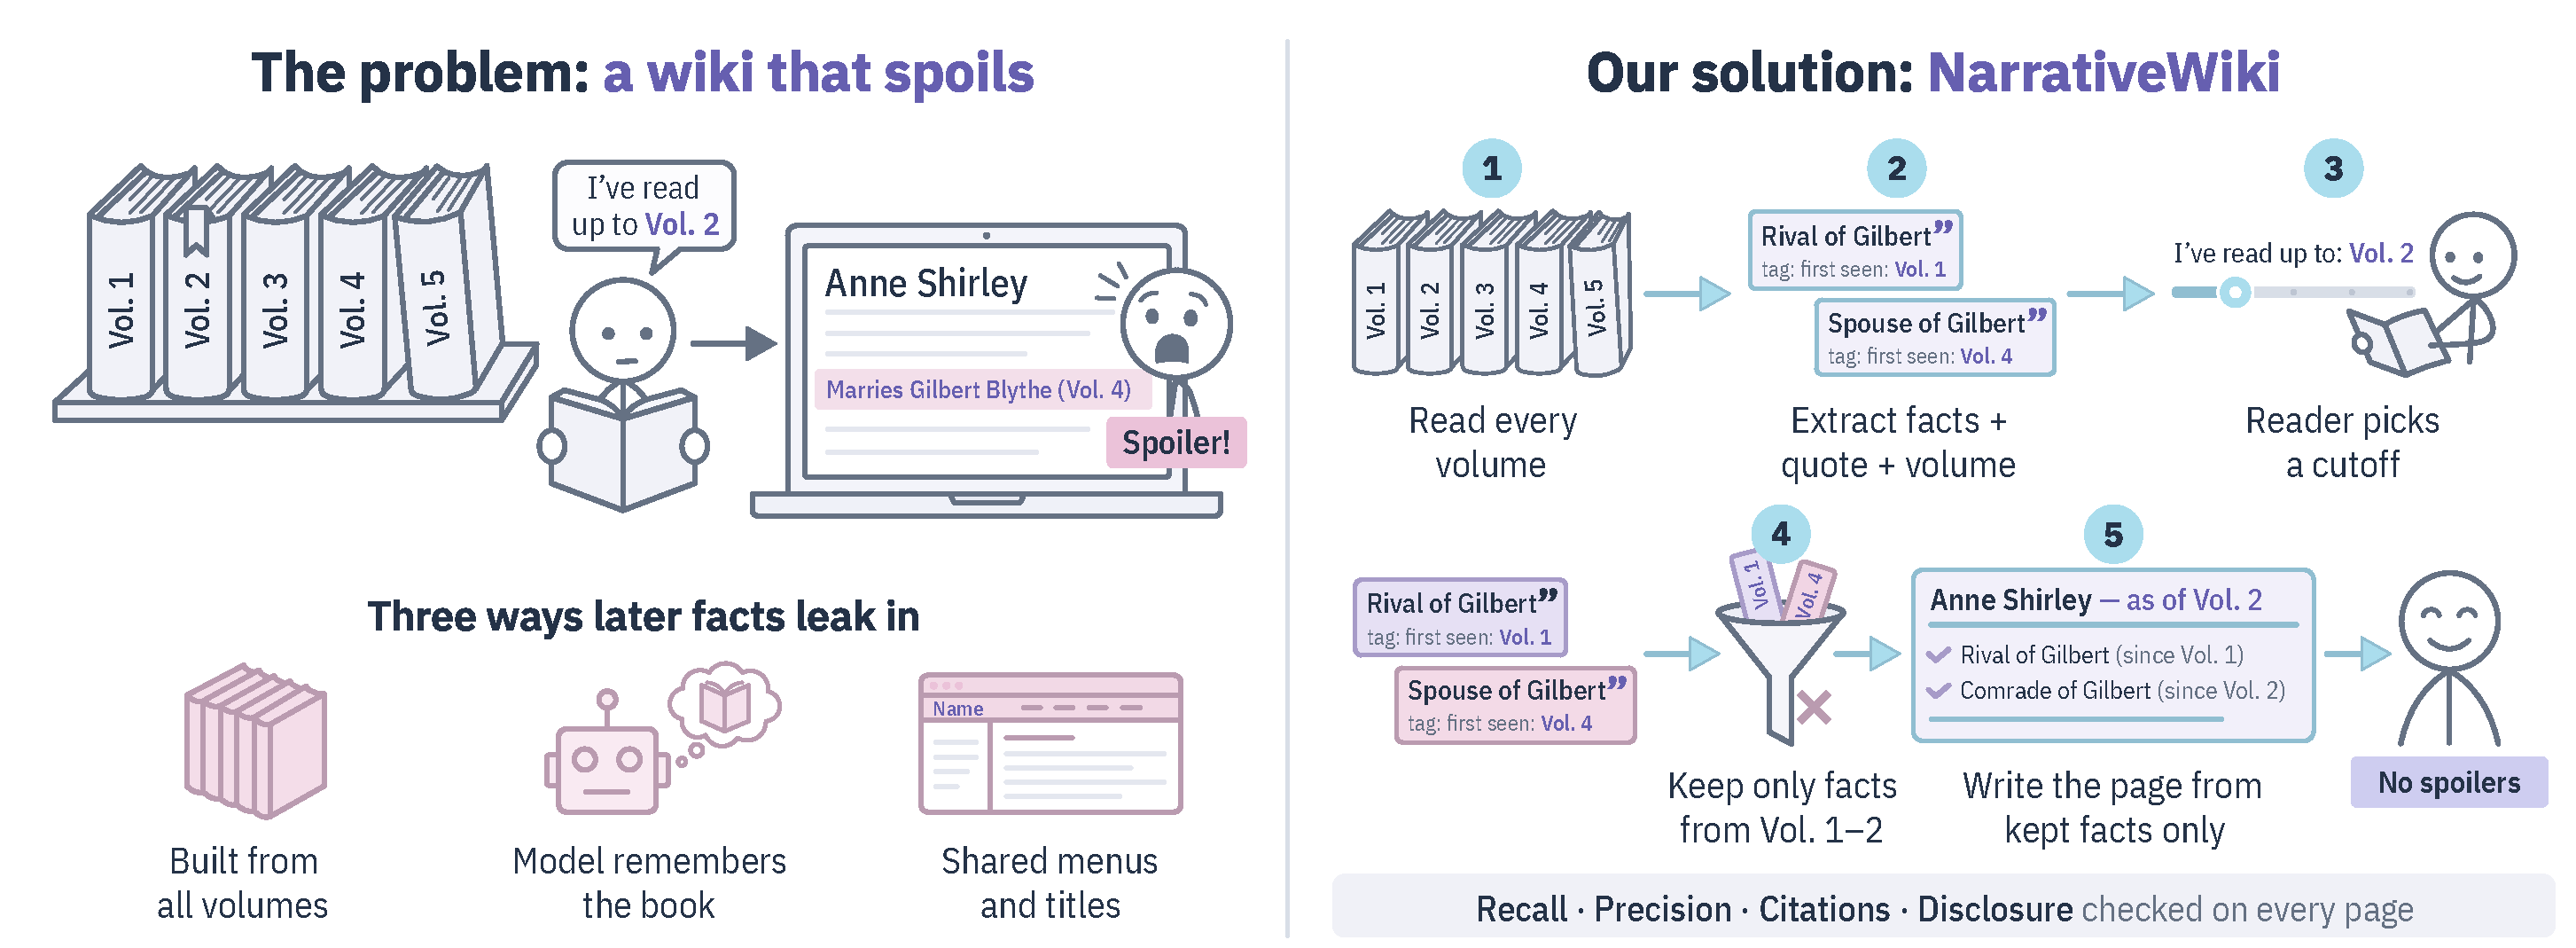
\includegraphics[width=\textwidth]{figures/f0-teaser.pdf}
\caption{Overview. Left: a whole-series wiki reveals Anne's marriage to Gilbert (volume~4)
to a reader at volume~2. Later information can enter through a full-series index, generator
memory or surfaces shared across cutoffs. Right: the intended cutoff mechanism of \sys,
which filters claims before generation. The illustration depicts the design goal rather
than an observed guarantee of spoiler-free output.}
\label{fig:overview}
\end{figure*}

\begin{figure}[t]
\centering
% F0 (teaser, one column): what a cutoff means, on real stored data. The four intervals are rows of
% the frozen graph for Anne and Gilbert Blythe: ENEMY_OF v1-v1, RIVAL_OF v1-, COMRADE_OF v2-,
% SPOUSE_OF v4- (data/anne@v2/04_graph/graph.db, the reported build; the first build stored the
% same four); the page lines are from
% dist/anne@v2/wiki/v02/relationships/anne-shirley--gilbert-blythe.md.
\begin{tikzpicture}[x=1.0cm, y=0.5cm, font=\scriptsize,
  vol/.style={draw=nwgray, fill=nwgraybg, rounded corners=1.5pt, minimum width=0.9cm, minimum height=0.4cm, inner sep=0pt},
  bar/.style={rounded corners=2pt, minimum height=0.28cm, inner sep=0pt, anchor=west},
  lab/.style={anchor=east, font=\figfont\ttfamily},
]
% volumes
\foreach \i in {1,...,5}{ \node[vol] (v\i) at (\i,0) {\textbf{Vol.~\i}}; }
\node[anchor=east, font=\figfont, text=nwgray, align=right] at (0.45,0) {volume};
% reader cutoff
\fill[nwredbg, opacity=0.6] (2.5,-0.95) rectangle (5.5,-6.05);
\draw[nwred!70!nwaccent, very thick, line cap=round] (2.5,0.75) -- (2.5,-6.05);
\node[fill=nwred, text=nwink, rounded corners=2pt, font=\figfont\bfseries, inner sep=2pt] at (2.5,1.3) {reader has finished Volume 2: cutoff $t{=}2$};
\node[text=nwink, font=\figfont\itshape, anchor=east] at (5.45,-5.65) {later text: withheld};
% intervals (stored first volume .. end)
\node[lab] at (0.45,-1.7) {ENEMY\_OF};
\node[bar, fill=nwgray!50, minimum width=0.9cm] at (0.55,-1.7) {};
\node[font=\figfont, text=nwgray, anchor=west] at (1.5,-1.7) {Vol.~1 only};
\node[lab] at (0.45,-2.8) {RIVAL\_OF};
\node[bar, fill=nwblue!75, minimum width=1.93cm] at (0.55,-2.8) {};
\node[bar, fill=nwblue!20, minimum width=2.95cm] at (2.52,-2.8) {};
\node[lab] at (0.45,-3.9) {COMRADE\_OF};
\node[bar, fill=nwgreen!75, minimum width=0.93cm] at (1.55,-3.9) {};
\node[bar, fill=nwgreen!20, minimum width=2.95cm] at (2.52,-3.9) {};
\node[lab] at (0.45,-5.0) {SPOUSE\_OF};
\node[bar, fill=nworange!28, draw=nworange, dashed, minimum width=1.93cm] at (3.55,-5.0) {};
\node[font=\figfont, text=nwaccent] at (4.52,-5.0) {evidence in Vol.~4};
% rendered page at t=2
\node[draw=nwblue!75!nwaccent, fill=nwbluebg, rounded corners=3pt, anchor=north west, text width=6.75cm, align=left, inner sep=4pt, font=\figfont]
  (page) at (-1.15,-6.6) {%
  {\scriptsize\bfseries\color{nwaccent}Cutoff-2 relationship page}\\[2pt]
  \textbf{Anne Shirley --- Gilbert Blythe}\\[2pt]
  \emph{Rival of}, since Vol.~1 \hfill{\ttfamily [v01:c17:p0036]}\\[1pt]
  \emph{Comrade of}, since Vol.~2 \hfill{\ttfamily [v02:c01:p0055]}\\[1pt]
  \emph{Previously: Enemy of}, until Vol.~1 \hfill{\ttfamily [v01:c15:p0051]}\\[2pt]
  {\color{nwaccent}\emph{Spouse of} is withheld from pages and links.}};
\end{tikzpicture}

\caption{Reading cutoffs for one character pair. Relation intervals open at their
first-evidence volume. The cutoff-2 wiki renders intervals opened by volume~2 and withholds
the marriage evidenced in volume~4. Citations use \texttt{v<volume>:c<chapter>:p<paragraph>}.}
\label{fig:cutoff}
\end{figure}

Filtering retrieved passages alone does not enforce this boundary. Full-series entity
resolution can expose an identity established only in a later volume; a generator can supply
memorized plot details; and shared menus, titles or search indexes can disclose later names.
We encountered all three channels during development. Even with an explicit cutoff
instruction, a generator given all five books wrote on Priscilla Grant's volume-two page
that she ``entered Redmond College in Kingsport'' alongside Anne, although their college
attendance first appears in book three (Appendix~\ref{app:casebook}).

Temporal knowledge boundaries have been studied for role-playing agents
\citep{ahn2024timechara}, for conversational agents gated to the narrative present
\citep{huang2025living}, and for character representations extracted from long narratives
\citep{gurung2024chiron}. We study a linked reference artifact at every cutoff and evaluate
coverage, support and disclosure across its delivered surfaces. The contribution is the
task and evaluation framework; \sys serves as a reference implementation. We provide:
\begin{itemize}[leftmargin=*,itemsep=1pt,topsep=2pt]
  \item \textbf{A task and threat model} for cutoff-bounded reference generation, covering
    pages, titles, links, navigation and search; gold facts dated by reveal volume; and three
    channels of later-information disclosure
    (Section~\ref{sec:task}).
  \item \textbf{An artifact-level evaluation protocol} applied to seven systems: assertions
    are enumerated across surfaces and sampled for precision and citation sufficiency;
    recall uses \res{T1-anne-gold-t5} gold facts; and disclosure search covers every page,
    with candidate sentences adjudicated and search recall tested on seeded cases
    (Section~\ref{sec:setup}). The pilot dataset documents corpus size, annotation units and
    illustrative records (Appendix~\ref{app:corpus}).
  \item \textbf{\sys}, a reference implementation that applies the cutoff to stored claims
    before page generation. One build yields a wiki for every cutoff (Figure~\ref{fig:overview}, right;
    Section~\ref{sec:method}).
  \item \textbf{A pilot comparison of cutoff designs.} On the original text, withholding
    later text from page generation yields no stated assessed later fact and \sys implies one by
    misreading eligible text (\res{M4-anne-total-cut} assessments;
    \res{M4-anne-total-cut-incl} including uncertain verdicts). Closed-book and full-text
    instruction disclose more. \sys has lower gold recall than long-context prompting,
    citation sufficiency of about one half and early pages shaped by later volumes\ifnwdecon{};
    on renamed, paraphrased text, it states a later marriage from a character's prediction\fi{}
    (Section~\ref{sec:results}).
\end{itemize}
